\documentclass{standalone}
\usepackage{tikz}
\usetikzlibrary{patterns, positioning}
\usepackage[sfdefault]{ClearSans} %% option 'sfdefault' activates Clear Sans as the default text font
\usepackage[T1]{fontenc}

\begin{document}
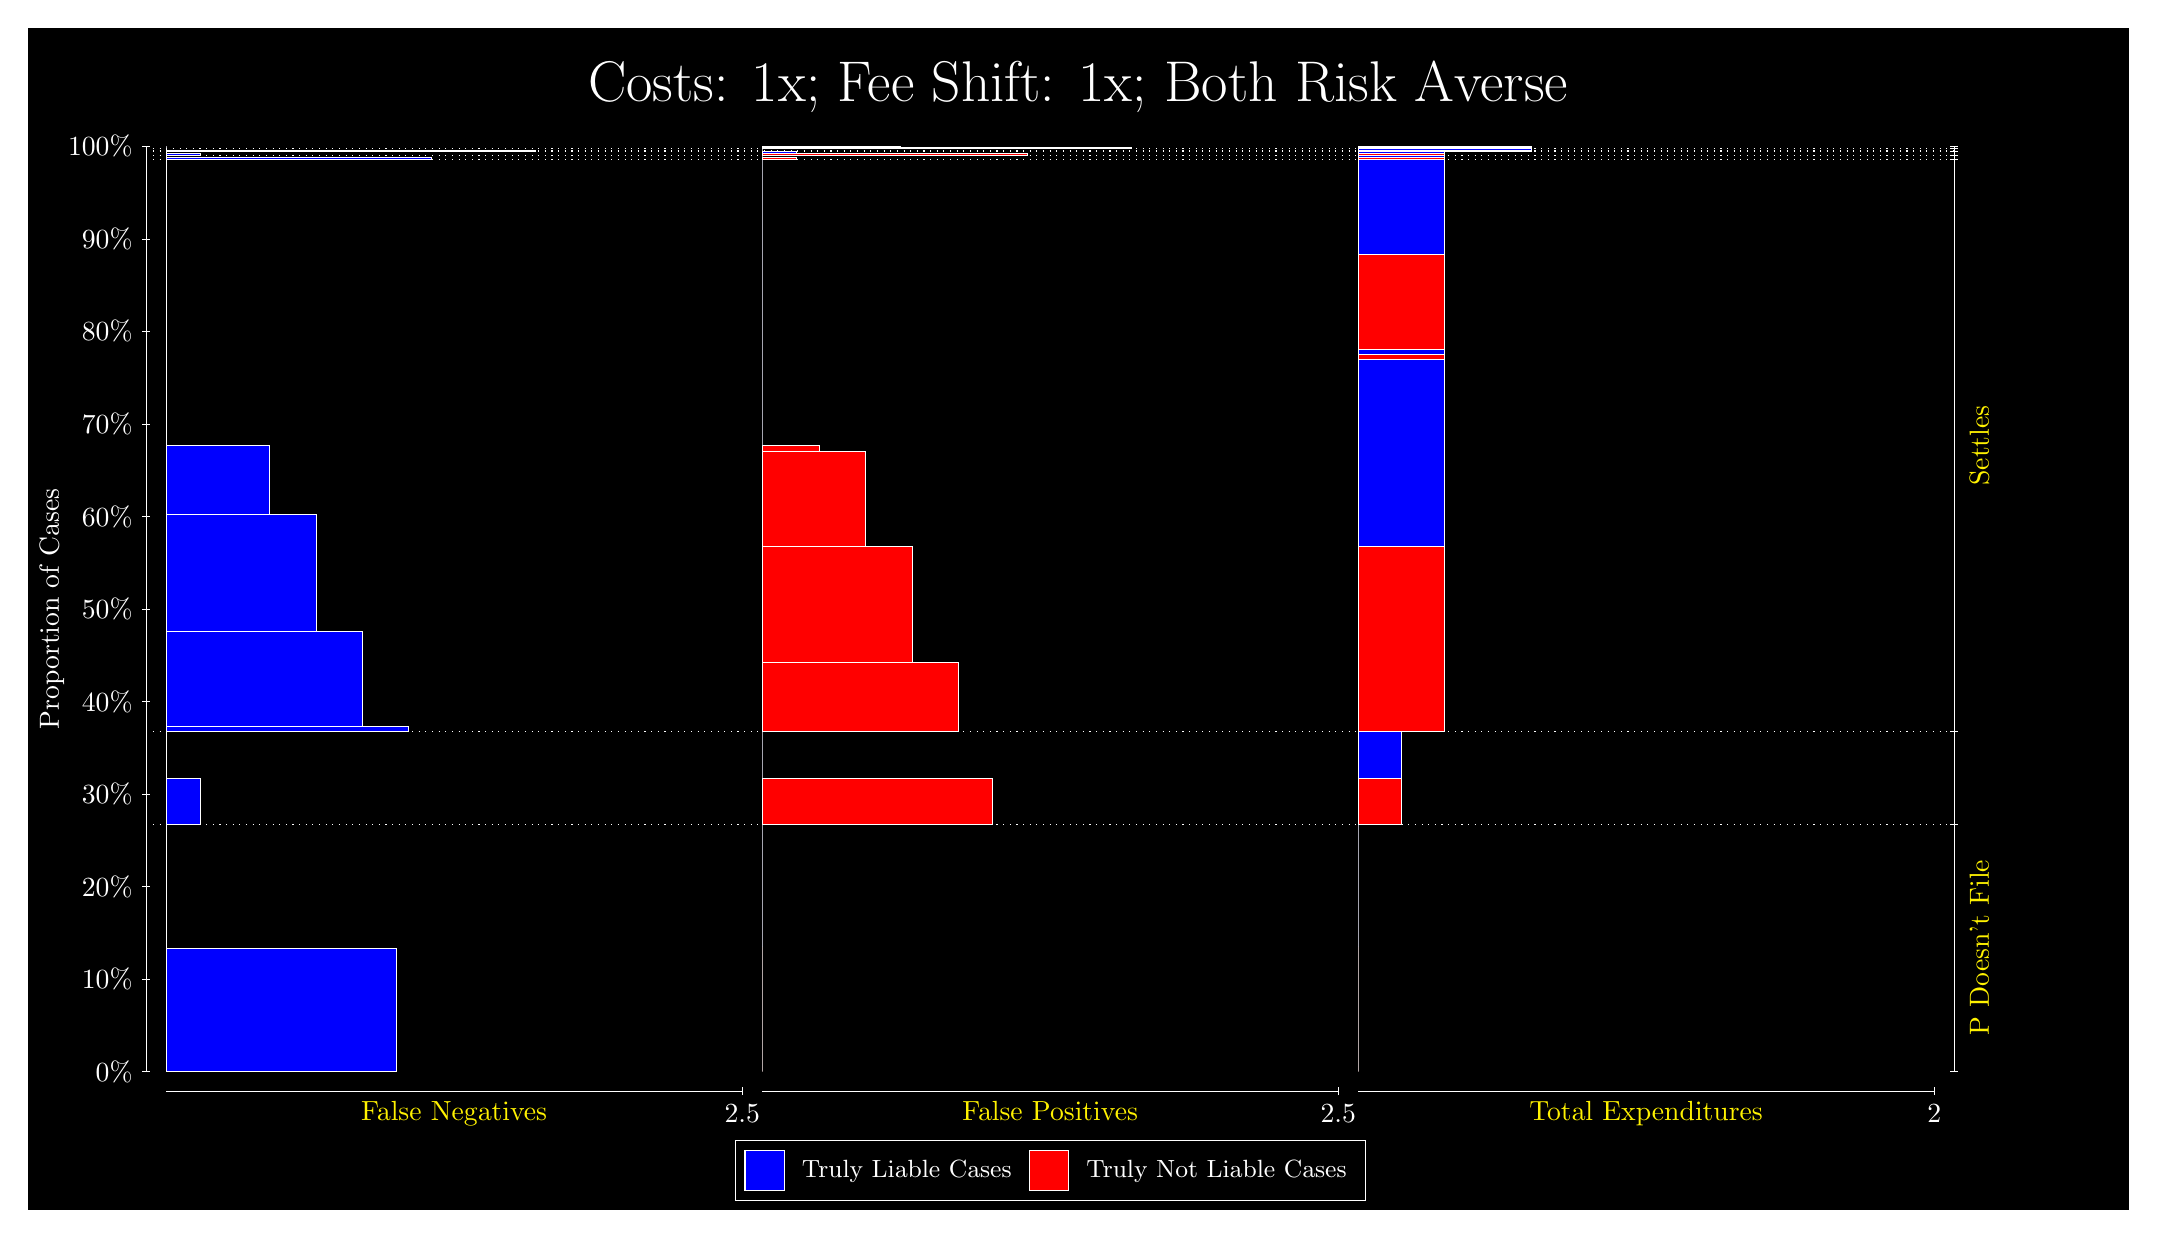
\begin{tikzpicture}
\draw[fill=black] (0,0) rectangle (26.667,15);
\draw[text=white] (0,13.5) rectangle (26.667,15) node[midway] {\huge Costs: 1x; Fee Shift: 1x; Both Risk Averse};
\draw[white, very thin] (1.5,1.75) -- (1.5,13.5);
\node[rotate=90, text=white, anchor=center] at (0.3, 7.625) {Proportion of Cases};
\draw[white, very thin] (1.45,1.75) -- (1.55,1.75);
\node[text=white, anchor=east] at (1.45, 1.75) {0\%};
\draw[white, very thin] (1.45,2.925) -- (1.55,2.925);
\node[text=white, anchor=east] at (1.45, 2.925) {10\%};
\draw[white, very thin] (1.45,4.1) -- (1.55,4.1);
\node[text=white, anchor=east] at (1.45, 4.1) {20\%};
\draw[white, very thin] (1.45,5.275) -- (1.55,5.275);
\node[text=white, anchor=east] at (1.45, 5.275) {30\%};
\draw[white, very thin] (1.45,6.45) -- (1.55,6.45);
\node[text=white, anchor=east] at (1.45, 6.45) {40\%};
\draw[white, very thin] (1.45,7.625) -- (1.55,7.625);
\node[text=white, anchor=east] at (1.45, 7.625) {50\%};
\draw[white, very thin] (1.45,8.8) -- (1.55,8.8);
\node[text=white, anchor=east] at (1.45, 8.8) {60\%};
\draw[white, very thin] (1.45,9.975) -- (1.55,9.975);
\node[text=white, anchor=east] at (1.45, 9.975) {70\%};
\draw[white, very thin] (1.45,11.15) -- (1.55,11.15);
\node[text=white, anchor=east] at (1.45, 11.15) {80\%};
\draw[white, very thin] (1.45,12.325) -- (1.55,12.325);
\node[text=white, anchor=east] at (1.45, 12.325) {90\%};
\draw[white, very thin] (1.45,13.5) -- (1.55,13.5);
\node[text=white, anchor=east] at (1.45, 13.5) {100\%};

\draw[white, very thin] (24.457,1.75) -- (24.457,13.5);
\draw[white, very thin] (24.407,1.75) -- (24.507,1.75);
\node[anchor=west] at (24.407, 1.75) {};
\draw[white, very thin] (24.407,4.8922) -- (24.507,4.8922);
\node[anchor=west] at (24.407, 4.8922) {};
\draw[white, very thin] (24.407,6.0672) -- (24.507,6.0672);
\node[anchor=west] at (24.407, 6.0672) {};
\draw[white, very thin] (24.407,13.334) -- (24.507,13.334);
\node[anchor=west] at (24.407, 13.334) {};
\draw[white, very thin] (24.407,13.382) -- (24.507,13.382);
\node[anchor=west] at (24.407, 13.382) {};
\draw[white, very thin] (24.407,13.441) -- (24.507,13.441);
\node[anchor=west] at (24.407, 13.441) {};
\draw[white, very thin] (24.407,13.47) -- (24.507,13.47);
\node[anchor=west] at (24.407, 13.47) {};
\draw[white, very thin] (24.407,13.5) -- (24.507,13.5);
\node[anchor=west] at (24.407, 13.5) {};

\draw[white, very thin, fill=blue] (1.75,1.75) rectangle (4.6775,3.3106);
\draw[white, very thin, fill=red] (1.75,3.3106) rectangle (1.75,4.8922);
\draw[white, very thin, fill=blue] (1.75,4.8922) rectangle (2.1891,5.4797);
\draw[white, very thin, fill=red] (1.75,5.4797) rectangle (1.75,6.0672);
\draw[white, very thin, fill=blue] (1.75,6.0672) rectangle (4.8239,6.1329);
\draw[white, very thin, fill=blue] (1.75,6.1329) rectangle (4.2384,7.3395);
\draw[white, very thin, fill=blue] (1.75,7.3395) rectangle (3.6529,8.8218);
\draw[white, very thin, fill=blue] (1.75,8.8218) rectangle (3.0674,9.7031);
\draw[white, very thin, fill=red] (1.75,9.7031) rectangle (1.75,13.334);
\draw[white, very thin, fill=blue] (1.75,13.334) rectangle (5.1167,13.358);
\draw[white, very thin, fill=red] (1.75,13.358) rectangle (1.75,13.382);
\draw[white, very thin, fill=blue] (1.75,13.382) rectangle (2.1891,13.418);
\draw[white, very thin, fill=red] (1.75,13.418) rectangle (1.75,13.441);
\draw[white, very thin, fill=blue] (1.75,13.441) rectangle (6.4341,13.456);
\draw[white, very thin, fill=red] (1.75,13.456) rectangle (1.75,13.47);
\draw[white, very thin, fill=red] (1.75,13.47) rectangle (1.75,13.483);
\draw[white, very thin, fill=blue] (1.75,13.483) rectangle (1.75,13.5);
\draw[white, very thin, fill=red] (9.3189,1.75) rectangle (9.3189,3.3316);
\draw[white, very thin, fill=blue] (9.3189,3.3316) rectangle (9.3189,4.8922);
\draw[white, very thin, fill=red] (9.3189,4.8922) rectangle (12.246,5.4797);
\draw[white, very thin, fill=blue] (9.3189,5.4797) rectangle (9.3189,6.0672);
\draw[white, very thin, fill=red] (9.3189,6.0672) rectangle (11.807,6.9485);
\draw[white, very thin, fill=red] (9.3189,6.9485) rectangle (11.222,8.4268);
\draw[white, very thin, fill=red] (9.3189,8.4268) rectangle (10.636,9.6269);
\draw[white, very thin, fill=red] (9.3189,9.6269) rectangle (10.051,9.698);
\draw[white, very thin, fill=blue] (9.3189,9.698) rectangle (9.3189,13.334);
\draw[white, very thin, fill=red] (9.3189,13.334) rectangle (9.758,13.358);
\draw[white, very thin, fill=blue] (9.3189,13.358) rectangle (9.3189,13.382);
\draw[white, very thin, fill=red] (9.3189,13.382) rectangle (12.686,13.406);
\draw[white, very thin, fill=blue] (9.3189,13.406) rectangle (9.758,13.441);
\draw[white, very thin, fill=red] (9.3189,13.441) rectangle (9.3189,13.456);
\draw[white, very thin, fill=blue] (9.3189,13.456) rectangle (9.3189,13.47);
\draw[white, very thin, fill=red] (9.3189,13.47) rectangle (14.003,13.483);
\draw[white, very thin, fill=blue] (9.3189,13.483) rectangle (11.075,13.5);
\draw[white, very thin, fill=red] (16.888,1.75) rectangle (16.888,3.3316);
\draw[white, very thin, fill=blue] (16.888,3.3316) rectangle (16.888,4.8922);
\draw[white, very thin, fill=red] (16.888,4.8922) rectangle (17.437,5.4797);
\draw[white, very thin, fill=blue] (16.888,5.4797) rectangle (17.437,6.0672);
\draw[white, very thin, fill=red] (16.888,6.0672) rectangle (17.986,8.4268);
\draw[white, very thin, fill=blue] (16.888,8.4268) rectangle (17.986,10.79);
\draw[white, very thin, fill=red] (16.888,10.79) rectangle (17.986,10.862);
\draw[white, very thin, fill=blue] (16.888,10.862) rectangle (17.986,10.927);
\draw[white, very thin, fill=red] (16.888,10.927) rectangle (17.986,12.127);
\draw[white, very thin, fill=blue] (16.888,12.127) rectangle (17.986,13.334);
\draw[white, very thin, fill=red] (16.888,13.334) rectangle (17.986,13.358);
\draw[white, very thin, fill=blue] (16.888,13.358) rectangle (17.986,13.382);
\draw[white, very thin, fill=red] (16.888,13.382) rectangle (17.986,13.406);
\draw[white, very thin, fill=blue] (16.888,13.406) rectangle (17.986,13.441);
\draw[white, very thin, fill=red] (16.888,13.441) rectangle (19.083,13.456);
\draw[white, very thin, fill=blue] (16.888,13.456) rectangle (19.083,13.47);
\draw[white, very thin, fill=red] (16.888,13.47) rectangle (19.083,13.483);
\draw[white, very thin, fill=blue] (16.888,13.483) rectangle (19.083,13.5);
\draw[white, dotted] (1.5,4.8922) -- (24.457,4.8922);
\draw[white, dotted] (1.5,6.0672) -- (24.457,6.0672);
\draw[white, dotted] (1.5,13.334) -- (24.457,13.334);
\draw[white, dotted] (1.5,13.382) -- (24.457,13.382);
\draw[white, dotted] (1.5,13.441) -- (24.457,13.441);
\draw[white, dotted] (1.5,13.47) -- (24.457,13.47);
\draw[white, very thin] (1.75,1.5) -- (9.0689,1.5);
\node[text=yellow, anchor=north] at (5.4094, 1.5) {False Negatives};
\draw[white, very thin] (9.0689,1.45) -- (9.0689,1.55);
\node[text=white, anchor=north] at (9.0689, 1.45) {2.5};

\draw[white, very thin] (9.3189,1.5) -- (16.638,1.5);
\node[text=yellow, anchor=north] at (12.978, 1.5) {False Positives};
\draw[white, very thin] (16.638,1.45) -- (16.638,1.55);
\node[text=white, anchor=north] at (16.638, 1.45) {2.5};

\draw[white, very thin] (16.888,1.5) -- (24.207,1.5);
\node[text=yellow, anchor=north] at (20.547, 1.5) {Total Expenditures};
\draw[white, very thin] (24.207,1.45) -- (24.207,1.55);
\node[text=white, anchor=north] at (24.207, 1.45) {2};

\node[text=yellow, centered, rotate=90] at (24.777, 3.3211) {P Doesn't File};

\node[text=yellow, centered, rotate=90] at (24.777, 9.7005) {Settles};





\draw (12.978300999999998,1.5) node[draw=none] (baseCoordinate) {};
\begin{scope}[align=center]
        \matrix[scale=0.5, draw=white, below=0.5cm of baseCoordinate, nodes={draw}, column sep=0.1cm]{
            \node[rectangle, draw, minimum width=0.5cm, minimum height=0.5cm, fill=blue] {}; &
            \node[draw=none, font=\small, text=white] (B) {Truly Liable Cases}; &
            \node[rectangle, draw, minimum width=0.5cm, minimum height=0.5cm, fill=red] {}; &
            \node[draw=none, font=\small, text=white] (B) {Truly Not Liable Cases}; \\
            };
\end{scope}

\end{tikzpicture}
\end{document}